\begin{figure}[t]
\centering
% Round 20 built the bar ranking (lower panel). Round 31 added the upper panel: two
% independent reviewers said the composition finding was buried under the auditing
% machinery, and the depth ladder that IS the finding existed only as an appendix
% table (tab:deep_composition) while the body printed one endpoint. Values are that
% table's rows verbatim -- singles-only, depth-8-in-library, and sup F_3.
% Bars are the PAIRED costs against the depth-8-in-library arm; the primitive row
% shows the per-arm SPAN because the pooled +0.664 hides that `commute` is by far
% the cheapest to hold out. Natural width ~13.2cm, so \resizebox scales by ~1.0 --
% re-render and LOOK at the page after any change; a collision here is invisible
% to every text-based gate.
\resizebox{0.88\textwidth}{!}{%
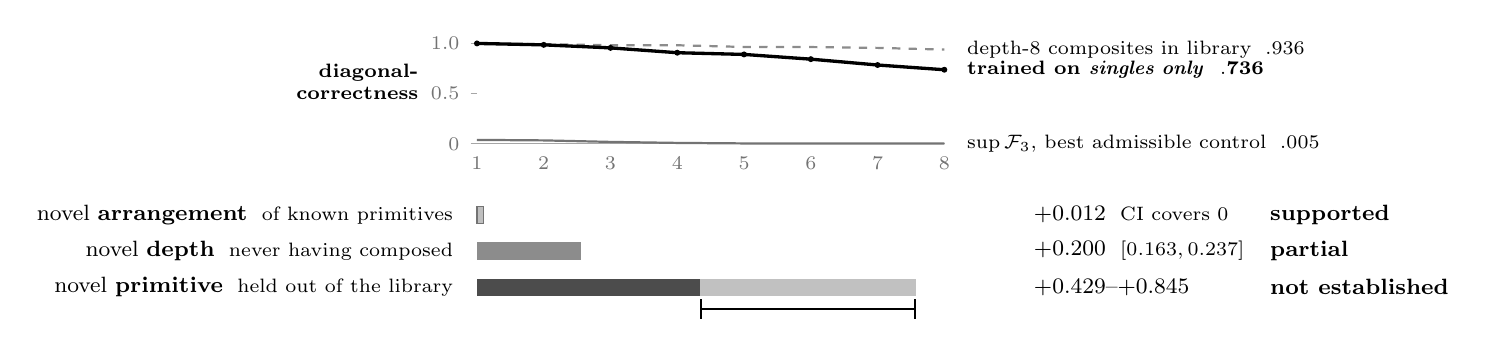
\begin{tikzpicture}[font=\footnotesize]
\def\s{6.6}          % cm per 1.0 of paired cost (lower panel)
\def\vx{6.95}        % value column
\def\wx{9.95}        % verdict column -- must clear the widest value string
\def\py{0.90}        % upper panel: y of value 0.0
\def\ph{1.28}        % upper panel: height of the full 0..1 range
\def\dx{0.848}       % upper panel: x step per depth level (8 levels span 0..5.94)

% ================= upper panel: the depth ladder =================
% Full 0..1 axis: the distance between the learned arms and the admissible
% ceiling IS the evidence, so it is drawn rather than described.
\draw[black!35] (0,\py) -- (5.94,\py);
\foreach \v/\lab in {0/0, 0.5/0.5, 1/1.0} {
  \draw[black!35] (-0.08, {\py+\ph*\v}) -- (0, {\py+\ph*\v});
  \node[anchor=east, font=\scriptsize, black!55] at (-0.10, {\py+\ph*\v}) {\lab};
}
\foreach \d in {1,...,8} {
  \node[anchor=north, font=\scriptsize, black!55] at ({(\d-1)*\dx}, {\py-0.04}) {\d};
}

\draw[black!45, dashed, thick]
  (0.0,2.1736) -- (0.848,2.1659) -- (1.696,2.1544) -- (2.544,2.1531) -- (3.392,2.1314) -- (4.24,2.1301) -- (5.088,2.1198) -- (5.936,2.0981);
\draw[black, very thick]
  (0.0,2.1762) -- (0.848,2.1582) -- (1.696,2.1198) -- (2.544,2.0584) -- (3.392,2.0366) -- (4.24,1.9765) -- (5.088,1.9022) -- (5.936,1.8421);
\foreach \x/\y in {0.0/2.1762, 0.848/2.1582, 1.696/2.1198, 2.544/2.0584, 3.392/2.0366, 4.24/1.9765, 5.088/1.9022, 5.936/1.8421}
  { \fill (\x,\y) circle (0.038); }
\draw[black!55, thick]
  (0.0,0.9512) -- (0.848,0.9448) -- (1.696,0.9256) -- (2.544,0.9128) -- (3.392,0.9064) -- (4.24,0.9064) -- (5.088,0.9064) -- (5.936,0.9064);

\node[anchor=west, font=\scriptsize] at (6.10,2.0981) {depth-8 composites in library \;$.936$};
\node[anchor=west, font=\scriptsize\bfseries] at (6.10,1.8421) {trained on \emph{singles only} \;$\mathbf{.736}$};
\node[anchor=west, font=\scriptsize] at (6.10,0.9064) {$\sup\mathcal{F}_3$, best admissible control \;$.005$};
\node[anchor=east, font=\scriptsize\bfseries, align=right] at (-0.62,{\py+0.62*\ph}) {diagonal-\\correctness};

% ================= lower panel: the three costs =================
% ---------- arrangement ----------
\node[anchor=east] at (-0.18, 0) {novel \textbf{arrangement} \;{\scriptsize of known primitives}};
\fill[black!25] (0, -0.11) rectangle ++(0.012*\s, 0.22);
\draw[black!55] (0, -0.11) rectangle ++(0.012*\s, 0.22);
\node[anchor=west] at (\vx, 0) {$+0.012$ \;{\scriptsize CI covers $0$}};
\node[anchor=west, font=\footnotesize\bfseries] at (\wx, 0) {supported};

% ---------- depth ----------
\node[anchor=east] at (-0.18, -0.46) {novel \textbf{depth} \;{\scriptsize never having composed}};
\fill[black!45] (0, -0.57) rectangle ++(0.200*\s, 0.22);
\node[anchor=west] at (\vx, -0.46) {$+0.200$ \;{\scriptsize $[0.163,0.237]$}};
\node[anchor=west, font=\footnotesize\bfseries] at (\wx, -0.46) {partial};

% ---------- primitive ----------
\node[anchor=east] at (-0.18, -0.92) {novel \textbf{primitive} \;{\scriptsize held out of the library}};
\fill[black!70] (0, -1.03) rectangle ++(0.429*\s, 0.22);
\fill[black!70, opacity=0.35] (0.429*\s, -1.03) rectangle ++({(0.845-0.429)*\s}, 0.22);
\draw[|-|, thick] (0.429*\s, -1.20) -- (0.845*\s, -1.20);
\node[anchor=west] at (\vx, -0.92) {$+0.429$--$+0.845$};
\node[anchor=west, font=\footnotesize\bfseries] at (\wx, -0.92) {not established};

\end{tikzpicture}}
\caption{\textbf{Takeaway: diagonal-correctness (\S\ref{sec:method}) decays gracefully with composition depth, and novel
\emph{arrangement} is nearly free where a novel \emph{primitive} is fatal.} \textbf{Below}: paired drops at
$d{=}8$ against that covered arm; the primitive span pools to $+0.664$; \textbf{the arrangement bar
% Round 53's cold-reconstruction read, and the round's own defect class caught one page late:
% tab:composition_matrix_full -- captioned "The complete training-depth x test-depth matrix", which is
% EXACTLY the grid this round's reviewer sketched in their SS19 -- was referenced from ZERO body files
% (measured: `grep -c "app:composition}"' over all six, plus this caption, returns 0 everywhere), and
% its enclosing appendix AH opens "Superseded, and kept only for continuity ... a reader checking the
% current claims can skip to AU".  So the paper told the reviewer to skip the section holding their
% answer.  check_protected_claims.py's UNCITED_OK was satisfied throughout: the table IS cited, five
% times, all of them from other appendices.  THE GATE CHECKED CITEDNESS, NOT REACHABILITY FROM THE BODY.
%   This line is the fix's body half, and it is height-free: the caption's last rendered line carried
% 146.76pt of tail (~39 characters) and the addition renders as "; exposure x depth in full: AH", 30.
% No number is added, so check_caption_rows.py gains no obligation.  Pinned by check_grid_route().
replicates on a second class set} (tags \texttt{r93},~\texttt{r94}; Appendices~\ref{app:deep_composition},~\ref{app:lopo},~\ref{app:order_diversity}; exposure~$\times$~depth in full: \ref{app:composition}).}
\label{fig:novelty_cost}
\end{figure}
